\chapter{Spatial Partitioning}
\label{ch:geometric_data_structures}

Geometric algorithms depend on data structures that organize points, lines,
regions, and higher-dimensional objects for efficient construction and query.
This chapter presents hierarchical and ordered structures for spatial
searching: KD-trees, quadtrees, R-trees, interval trees, and segment trees.
Together they support nearest-neighbor queries, range searching, collision
detection, intersection reporting, and other geometric operations.
\label{ch:spatial_structures}

\section{K-Dimensional Trees}
\label{sec:kd_tree}

\subsection{1. Overview}
A \textbf{KD-tree}\index{KD-tree} is a space-partitioning\index{space-partitioning} data structure for organizing points in a $k$-dimensional space~\cite{bentley1975}. It is a binary tree where every node is a $k$-dimensional point and every non-leaf node represents a splitting hyperplane. This structure is extremely efficient for range searches and nearest neighbor queries in low-to-medium dimensional spaces. A first treatment of k-d trees in the context of orthogonal range queries appears in Section~\ref{sec:rangesearch_kd_trees}; this section gives the full data structure, including construction, balancing, and query pruning.

\subsection{2. Definitions}
\begin{definition}[Splitting Hyperplane]
\label{def:kd_splitting_hyperplane}
A \emph{splitting hyperplane} is a $(k-1)$-dimensional surface that divides the point set into two subsets. It is always perpendicular to one of the coordinate axes.
\end{definition}

\begin{definition}[Depth]
\label{def:kd_depth}
The \emph{depth} $d$ of a node is its level in the tree. The splitting axis is chosen as $\text{axis} = d \bmod k$.
\end{definition}

\begin{definition}[KD-tree Median]
\label{def:kd_median}
The \emph{median} is the point chosen to split the set at each node, ensuring the tree is balanced. Choosing the exact median guarantees that both subtrees contain at most $\lfloor n/2 \rfloor$ points.
\end{definition}

\begin{definition}[Bounding Box]
\label{def:kd_bounding_box}
The \emph{bounding box} of a node is the region of space represented by that node and all its descendants. At depth $d$, the bounding box is an axis-aligned rectangle restricted along axis $d \bmod k$ to at most one side of the splitting hyperplane.
\end{definition}

\subsection{3. Theory}
A KD-tree is built by recursively partitioning the set of points. At each level, the algorithm chooses one of the $k$ dimensions and splits the points into two groups: those whose coordinate in that dimension is less than the median and those whose coordinate is greater.

\begin{theorem}[KD-tree Construction Complexity]
\label{thm:kd_build_complexity}
Building a KD-tree on $n$ points in $\mathbb{R}^k$ takes $O(n \log n)$ time when using a linear-time median selection algorithm at each level, and $O(n k \log n)$ time when sorting at each level.
\end{theorem}
\begin{proof}
At each level of recursion we partition at most $n$ points. If we use an $O(n)$ median-finding algorithm (e.g., quickselect), the total work at level $i$ is $O(n)$, and the tree has $O(\log n)$ levels (assuming balanced splits), giving $O(n \log n)$ total. With sorting, each level costs $O(n \log n)$ for a total of $O(n \log^2 n)$, but a pre-sorted approach or median-of-medians reduces this to $O(n \log n)$.
\end{proof}

For \textbf{Nearest Neighbor Search}\index{nearest neighbor search}, the tree is traversed from the root down to the leaf containing the query point. The distance from the query to this leaf is our initial ``best'' distance. Then, the algorithm backtracks up the tree, checking if any other branches could contain a closer point. This is done by checking if the query point's distance to a node's splitting hyperplane is smaller than the current best distance.

\begin{theorem}[KD-tree Nearest Neighbor Search]
\label{thm:kd_nn_complexity}
For $n$ points in $\mathbb{R}^k$ with fixed $k$, the expected nearest neighbor search time in a randomly built KD-tree is $O(\log n)$.
\end{theorem}
\begin{proof}
The expected number of nodes visited during a nearest neighbor query is $O(2^k \log n)$ for uniformly distributed points~\cite{friedman1977}. For fixed $k$, this simplifies to $O(\log n)$. The key insight is that the pruning criterion---skipping a subtree when the splitting hyperplane is farther than the current best---eliminates most branches. In the worst case (e.g., all points equidistant from the query), no pruning occurs and $O(n)$ nodes are visited.
\end{proof}

\begin{example}[KD-tree Construction in $\mathbb{R}^2$]
\label{ex:kd_build}
Consider the point set $S = \{(2,3),\ (5,4),\ (9,6),\ (4,7),\ (8,1),\ (7,2)\}$.
\begin{enumerate}
    \item \textbf{Root (depth $0$, axis $x$):} Median $x$-coordinate is $5$ (from sorted $x$: $2,4,5,7,8,9$).  Node: $(5,4)$.  Left subtree: $\{(2,3),(4,7)\}$; right subtree: $\{(9,6),(8,1),(7,2)\}$.
    \item \textbf{Left child (depth $1$, axis $y$):} Median $y$-coordinate of $\{(2,3),(4,7)\}$ is $3$ or $7$.  Node: $(2,3)$.  Right child: $(4,7)$.
    \item \textbf{Right child (depth $1$, axis $y$):} Median $y$-coordinate of $\{(9,6),(8,1),(7,2)\}$ is $2$.  Node: $(7,2)$.  Left child: $(8,1)$; right child: $(9,6)$.
\end{enumerate}
The resulting tree partitions $\mathbb{R}^2$ into rectangular regions, each containing exactly one point.
\end{example}

\begin{figure}[htbp]
\centering
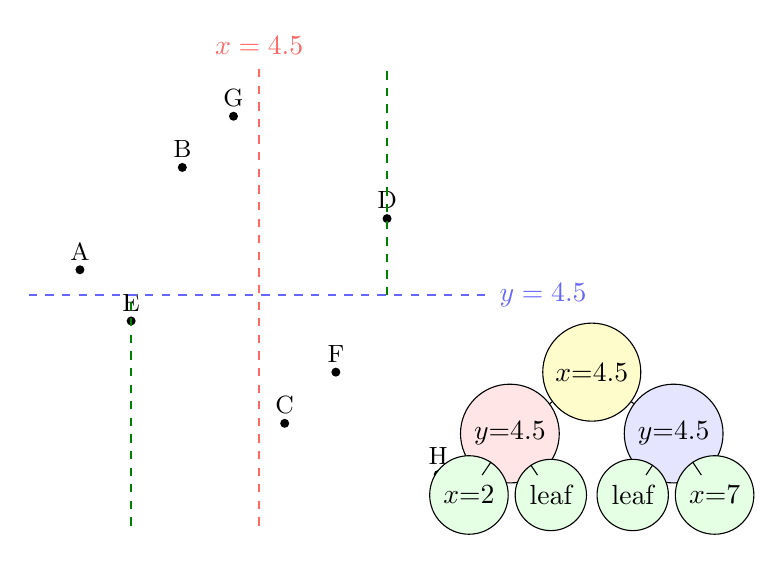
\begin{tikzpicture}[scale=0.65]
  \foreach \p/\l in {(1,5)/A, (3,7)/B, (5,2)/C, (7,6)/D, (2,4)/E, (6,3)/F, (4,8)/G, (8,1)/H} {
    \fill \p circle (2.5pt) node[above] {\small \l};
  }
  \draw[red!60,thick,dashed] (4.5,0)--(4.5,9) node[above] {$x=4.5$};
  \draw[blue!60,thick,dashed] (0,4.5)--(9,4.5) node[right] {$y=4.5$};
  \draw[green!50!black,thick,dashed] (2,0)--(2,4.5);
  \draw[green!50!black,thick,dashed] (7,4.5)--(7,9);
  \begin{scope}[xshift=11cm,yshift=3cm,scale=0.8]
    \node[draw,circle,fill=yellow!20] (root) at (0,0) {$x{=}4.5$};
    \node[draw,circle,fill=red!10] (l) at (-2,-1.5) {$y{=}4.5$};
    \node[draw,circle,fill=blue!10] (r) at (2,-1.5) {$y{=}4.5$};
    \node[draw,circle,fill=green!10] (ll) at (-3,-3) {$x{=}2$};
    \node[draw,circle,fill=green!10] (lr) at (-1,-3) {leaf};
    \node[draw,circle,fill=green!10] (rl) at (1,-3) {leaf};
    \node[draw,circle,fill=green!10] (rr) at (3,-3) {$x{=}7$};
    \draw (root)--(l) (root)--(r);
    \draw (l)--(ll) (l)--(lr);
    \draw (r)--(rl) (r)--(rr);
  \end{scope}
\end{tikzpicture}
\caption{KD-tree: (left) recursive axis-aligned partitioning of 2D space; (right) the corresponding binary tree structure.}
\label{fig:kd_tree}
\end{figure}


\subsection{4. Pseudo code}
\begin{algorithm}
\begin{algorithmic}[1]
\Function{BuildKDTree}{points, depth=0}
\label{alg:kd_build}
    \If{not points}
        \State \Return None
    \EndIf
    
    \Comment{1. Choose splitting axis}
    \State $k \gets \text{len(points[0])}$
    \State $\text{axis} \gets \text{depth} \bmod k$
    
    \Comment{2. Sort points by axis and find median}
    \State Sort points by axis
    \State $\text{mid} \gets \text{len(points)} / 2$
    
    \Comment{3. Create node and recurse}
    \State $\text{node} \gets \text{Node(points[mid])}$
    \State $\text{node.left} \gets \text{BuildKDTree(points[:mid], depth + 1)}$
    \State $\text{node.right} \gets \text{BuildKDTree(points[mid+1:], depth + 1)}$
    
    \State \Return node
\EndFunction

\Function{NearestNeighbor}{root, query, depth=0, best=None}
\label{alg:kd_nn}
    \If{root is None}
        \State \Return best
    \EndIf
    
    \State $k \gets \text{len(query)}$
    \State $\text{axis} \gets \text{depth} \bmod k$
    
    \Comment{Update current best}
    \State $\text{dist} \gets \text{EuclideanDistance(root.point, query)}$
    \If{best is None or dist < EuclideanDistance(best.point, query)}
        \State $\text{best} \gets \text{root}$
    \EndIf
        
    \Comment{Choose branch}
    \State $\text{next\_branch} \gets \begin{cases} \text{root.left} & \text{if query[axis] < root.point[axis]} \\ \text{root.right} & \text{otherwise} \end{cases}$
    \State $\text{other\_branch} \gets \begin{cases} \text{root.right} & \text{if query[axis] < root.point[axis]} \\ \text{root.left} & \text{otherwise} \end{cases}$
    
    \Comment{Go down the chosen branch}
    \State $\text{best} \gets \text{NearestNeighbor(next\_branch, query, depth + 1, best)}$
    
    \Comment{Check if we need to explore the other branch}
    \If{$|\text{query[axis]} - \text{root.point[axis]}| < \text{EuclideanDistance(best.point, query)}$}
        \State $\text{best} \gets \text{NearestNeighbor(other\_branch, query, depth + 1, best)}$
    \EndIf
        
    \State \Return best
\EndFunction
\end{algorithmic}
\end{algorithm}

\subsection{5. Parameters Selections}
\begin{definition}[Dimension Cycling]
\label{def:kd_dimension_cycling}
\emph{Dimension cycling} is the strategy for choosing the splitting axis at each level of the KD-tree. The standard choice is $\texttt{d \% k}$, but choosing the dimension with the largest variance (spread) can lead to more efficient searches.
\end{definition}

\begin{definition}[Leaf Size]
\label{def:kd_leaf_size}
The \emph{leaf size} is the maximum number of points stored in a single leaf node. Storing a few points (e.g., 5--10) in each leaf instead of one reduces recursion depth and can improve cache performance.
\end{definition}

\subsection{6. Complexity}
\begin{theorem}[KD-tree Complexity Summary]
\label{thm:kd_complexity}
For $n$ points in $\mathbb{R}^k$:
\begin{enumerate}
    \item \textbf{Construction:} $O(n \log n)$ time and $O(n)$ space.
    \item \textbf{Nearest Neighbor Search:} $O(\log n)$ expected time for fixed $k$; $O(n)$ worst case.
    \item \textbf{Range Search:} $O(n^{1-1/k} + t)$ time for reporting $t$ points in a rectangular range, for $k \ge 2$~\cite{friedman1977}.
\end{enumerate}
\end{theorem}
\begin{proof}
Construction follows from the median-based partitioning argument (\cref{thm:kd_build_complexity}). The range search bound $O(n^{1-1/k}+t)$ is obtained by observing that at each level $i$, at most $O(2^{ki/k})$ nodes can straddle the query boundary, and summing over $O(\log n)$ levels yields the stated bound. The space is $O(n)$ since each point is stored in exactly one leaf.
\end{proof}

\begin{remark}
The ``curse of dimensionality'' causes the range search bound to degrade to $O(n)$ when $k$ is large (e.g., $k > 20$). In such regimes, alternative structures like locality-sensitive hashing or random-projection trees are preferred.
\end{remark}

\subsection{7. Usages}
\begin{itemize}
    \item \textbf{Computational Geometry}\index{computational geometry}: Fast point location and range searching.
    \item \textbf{Machine Learning}\index{machine learning}: K-Nearest Neighbors (KNN) classification and clustering.
    \item \textbf{Computer Graphics}\index{computer graphics}: Ray tracing (finding the first object a ray intersects) and photon mapping.
    \item \textbf{Data Compression}: Efficient representation of multidimensional datasets.
    \item \textbf{GIS}\index{GIS}: Finding the closest point of interest (e.g., ``find the nearest gas station'').
\end{itemize}

\subsection{8. Testing methods and Edge cases}
\begin{itemize}
    \item \textbf{Duplicate Points}: Ensure the tree correctly handles multiple points at the same coordinates.
    \item \textbf{Points on Boundaries}: Correctly assign points that lie exactly on a splitting hyperplane.
    \item \textbf{Empty Tree}: Handle $n=0$ cases gracefully.
    \item \textbf{Very High Dimensions}: The ``Curse of Dimensionality'' affects KD-trees ($k > 20$); performance should be monitored.
    \item \textbf{Skewed Data}: Test on points that are nearly collinear or form very narrow clusters.
\end{itemize}

\subsection{9. References}
\begin{itemize}
    \item Bentley, J. L. (1975). ``Multidimensional binary search trees used for associative searching''. Communications of the ACM.
    \item Friedman, J. H., Bentley, J. L., \& Finkel, R. A. (1977). ``An Algorithm for Finding Best Matches in Logarithmic Expected Time''. ACM Transactions on Mathematical Software.
    \item Samet, H. (2006). ``Foundations of Multidimensional and Metric Data Structures''. Morgan Kaufmann.
    \item Wikipedia: \href{https://en.wikipedia.org/wiki/K-d_tree}{k-d tree}
\end{itemize}

\section{Quadtrees}
\label{sec:quadtree}

\subsection{1. Overview}
A \textbf{quadtree}\index{quadtree} is a tree data structure in which each internal node has exactly four children. It is most commonly used to partition a two-dimensional space by recursively subdividing it into four quadrants (North-West, North-East, South-West, South-East)~\cite{finkel1974}. Quadtrees are the 2D equivalent of Octrees\index{octree} (used in 3D) and are essential for efficient spatial querying\index{spatial query}, image compression, and collision detection.

\subsection{2. Definitions}
\begin{definition}[Quadtree Root]
\label{def:qt_root}
The \emph{root} of a quadtree is the top-level node representing the entire bounding area.
\end{definition}

\begin{definition}[Quadtree Leaf]
\label{def:qt_leaf}
A \emph{leaf} is a node that contains actual data points or a uniform value and has no children.
\end{definition}

\begin{definition}[Quadrant]
\label{def:qt_quadrant}
A \emph{quadrant} is one of the four rectangular regions created by splitting a parent node's region in half along both the $x$ and $y$ axes. The four quadrants are denoted NW, NE, SW, and SE.
\end{definition}

\begin{definition}[Quadtree Capacity]
\label{def:qt_capacity}
The \emph{capacity} of a quadtree node is the maximum number of points a single node can hold before it must be split into four children.
\end{definition}

\subsection{3. Theory}
A quadtree is built by starting with a bounding box and inserting points one by one. If a point is inserted into a leaf node that is already at its capacity, the node ``subdivides'' into four children, and all points in the node are redistributed to the correct child.

\begin{theorem}[Quadtree Subdivision Property]
\label{thm:qt_subdivision}
When a quadtree node with capacity $c$ is subdivided, at most 4 nodes of depth $d+1$ are created, each covering exactly one quarter of the parent's area. After subdivision, each child contains at most $c$ of the original points.
\end{theorem}
\begin{proof}
By construction, the four quadrants partition the parent's bounding box into four disjoint rectangular regions whose union equals the parent region. Each of the original $c$ (or fewer) points in the parent falls into exactly one quadrant based on its coordinates, so no point is lost or duplicated.
\end{proof}

For \textbf{Range Querying}\index{range query} (e.g., finding all points within a circle or rectangle), the quadtree allows us to quickly discard entire branches of the tree if their bounding box does not intersect the query area. This pruning results in $O(\log n)$ performance for localized searches.

\begin{example}[Quadtree Insertion Trace]
\label{ex:qt_insert}
Consider a quadtree with capacity $c=1$ and bounding box $[0,8] \times [0,8]$.
\begin{enumerate}
    \item Insert $(2,3)$: Root is empty, store directly.
    \item Insert $(6,7)$: Root is at capacity, subdivide into four quadrants centered at $(4,4)$.  $(2,3)$ falls in SW, $(6,7)$ falls in NE.
    \item Insert $(5,1)$: Root subdivided, $(5,1)$ falls in SE quadrant (empty), stored there.
    \item Insert $(1,6)$: Falls in NW quadrant (empty), stored there.
\end{enumerate}
All four children now each hold one point, and no further subdivision is needed until a fifth point lands in an occupied quadrant.
\end{example}

\begin{figure}[htbp]
\centering
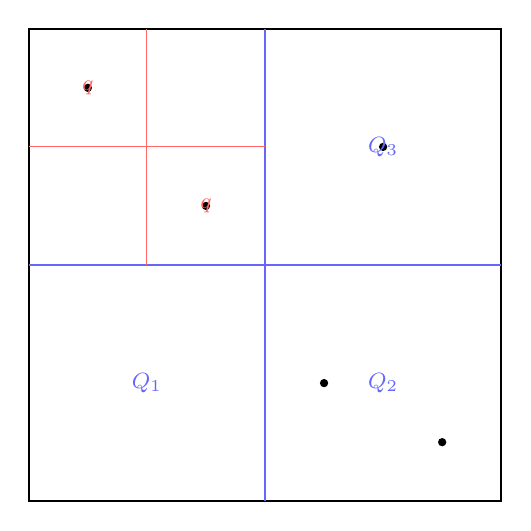
\begin{tikzpicture}[scale=0.75]
  \draw[thick] (0,0) rectangle (8,8);
  \draw[blue!60] (4,0)--(4,8);
  \draw[blue!60] (0,4)--(8,4);
  \draw[red!60] (2,4)--(2,8);
  \draw[red!60] (0,6)--(4,6);
  \fill (1,7) circle (2pt);
  \fill (3,5) circle (2pt);
  \fill (6,6) circle (2pt);
  \fill (5,2) circle (2pt);
  \fill (7,1) circle (2pt);
  \node[font=\footnotesize,blue!60] at (2,2) {$Q_1$};
  \node[font=\footnotesize,blue!60] at (6,2) {$Q_2$};
  \node[font=\footnotesize,blue!60] at (6,6) {$Q_3$};
  \node[font=\footnotesize,red!60] at (1,7) {$q$};
  \node[font=\footnotesize,red!60] at (3,5) {$q$};
\end{tikzpicture}
\caption{Quadtree: recursive 2D space partitioning. Quadrants with multiple points are subdivided; leaf quadrants contain at most one point.}
\label{fig:quadtree}
\end{figure}


\subsection{4. Pseudo code}
\begin{algorithm}
\begin{algorithmic}[1]
\Function{Insert}{node, point}
\label{alg:qt_insert}
    \If{not node.boundary.contains(point)}
        \State \Return False
    \EndIf
        
    \If{len(node.points) < node.capacity and not node.is\_divided}
        \State node.points.append(point)
        \State \Return True
    \EndIf
        
    \If{not node.is\_divided}
        \State node.subdivide()
    \EndIf
        
    \Comment{Try inserting into children}
    \If{node.nw.insert(point)}
        \State \Return True
    \EndIf
    \If{node.ne.insert(point)}
        \State \Return True
    \EndIf
    \If{node.sw.insert(point)}
        \State \Return True
    \EndIf
    \If{node.se.insert(point)}
        \State \Return True
    \EndIf
\EndFunction

\Function{Query}{node, range, result}
\label{alg:qt_query}
    \If{not node.boundary.intersects(range)}
        \State \Return
    \EndIf
        
    \Comment{Check points in current node}
    \For{p in node.points}
        \If{range.contains(p)}
            \State result.append(p)
        \EndIf
    \EndFor
        
    \Comment{Check children}
    \If{node.is\_divided}
        \State Query(node.nw, range, result)
        \State Query(node.ne, range, result)
        \State Query(node.sw, range, result)
        \State Query(node.se, range, result)
    \EndIf
\EndFunction
\end{algorithmic}
\end{algorithm}

\subsection{5. Parameters Selections}
\begin{definition}[Quadtree Node Capacity]
\label{def:qt_node_capacity}
The \emph{node capacity} is typically set to 4--16 points. Higher capacity reduces the number of internal nodes but increases the linear search time within each node.
\end{definition}

\begin{definition}[Maximum Depth]
\label{def:qt_max_depth}
The \emph{maximum depth} is a limit on subdivision to prevent infinite recursion in the case of overlapping or very dense points.
\end{definition}

\subsection{6. Complexity}
\begin{theorem}[Quadtree Complexity]
\label{thm:qt_complexity}
For $n$ uniformly distributed points in a quadtree with capacity $c$:
\begin{enumerate}
    \item \textbf{Construction:} $O(n \log n)$ on average; $O(n \cdot \text{depth})$ worst case for clustered data.
    \item \textbf{Range Query:} $O(\log n + t)$ for localized queries reporting $t$ points~\cite{samet1984}.
    \item \textbf{Space:} $O(n)$ on average, though internal node overhead can grow with depth.
\end{enumerate}
\end{theorem}

\begin{remark}
For highly non-uniform point distributions, quadtree depth can reach $O(n)$ in the worst case. Using a \textbf{point quadtree} variant (instead of region quadtree) or a loose quadtree can mitigate this.
\end{remark}

\subsection{7. Usages}
\begin{itemize}
    \item \textbf{Collision Detection}\index{collision detection}: Quickly finding pairs of objects that are close enough to collide.
    \item \textbf{Image Compression}\index{image compression}: Representing regions of uniform color with a single large node (e.g., in the TGA or PNG-like formats).
    \item \textbf{Video Games}: View frustum culling (rendering only objects that are visible within the camera's FOV).
    \item \textbf{GIS}\index{GIS}: Storing and querying map features like road networks or city locations.
    \item \textbf{Particle Systems}: Efficiently calculating local forces (e.g., gravity or repulsion) in many-body simulations.
\end{itemize}

\subsection{8. Testing methods and Edge cases}
\begin{itemize}
    \item \textbf{Uniform Point Distribution}: Verify that the tree divides evenly into a balanced structure.
    \item \textbf{Points on Boundaries}: Ensure points exactly on the dividing lines are assigned to exactly one child.
    \item \textbf{High-Density Clusters}: Ensure the ``capacity'' and ``max depth'' parameters prevent excessive subdivision.
    \item \textbf{Empty Areas}: Verify that large regions with no points are represented by a single empty leaf node.
    \item \textbf{Resizing}: Test if the quadtree can handle a dynamic bounding box or if it requires a fixed initial area.
\end{itemize}

\subsection{9. References}
\begin{itemize}
    \item Finkel, R. A., \& Bentley, J. L. (1974). ``Quad trees: A data structure for retrieval on composite keys''. Acta Informatica.
    \item Samet, H. (1984). ``The Quadtree and Related Hierarchical Data Structures''. ACM Computing Surveys.
    \item Samet, H. (2006). ``Foundations of Multidimensional and Metric Data Structures''. Morgan Kaufmann.
    \item Wikipedia: \href{https://en.wikipedia.org/wiki/Quadtree}{Quadtree}
\end{itemize}

\section{R-Trees}
\label{sec:r_tree}

\subsection{1. Overview}
An \textbf{R-tree}\index{R-tree} is a tree data structure used for efficient spatial indexing of multidimensional information, particularly objects represented as Minimum Bounding Rectangles (MBRs)~\cite{guttman1984}. Unlike KD-trees or quadtrees, which partition the space itself, R-trees group the objects into hierarchical, potentially overlapping regions. This makes R-trees exceptionally well-suited for disk-based databases and large-scale spatial datasets.

\subsection{2. Definitions}
\begin{definition}[Minimum Bounding Rectangle]
\label{def:rt_mbr}
The \emph{Minimum Bounding Rectangle (MBR)} of a node is the smallest rectangle (axis-aligned) that contains all the elements in that node's subtree.
\end{definition}

\begin{definition}[R-tree Leaf Node]
\label{def:rt_leaf}
A \emph{leaf node} stores pointers to the actual geometric objects and their MBRs.
\end{definition}

\begin{definition}[R-tree Internal Node]
\label{def:rt_internal}
An \emph{internal node} stores a pointer to a child node and the MBR of that child.
\end{definition}

\begin{definition}[R-tree Balance Property]
\label{def:rt_balance}
An R-tree is always \emph{height-balanced}: all leaf nodes appear at the same depth. This is analogous to the B-tree balance property.
\end{definition}

\subsection{3. Theory}
R-trees are built by grouping nearby objects and enclosing them in their MBR.
\begin{enumerate}
    \item \textbf{Insertion}: To insert an object, we start at the root and recursively choose a child node whose MBR requires the least expansion to include the new object.
    \item \textbf{Node Splitting}: When a node exceeds its capacity, it must be split into two. Since the choice of split affects search performance, heuristics are used to minimize the area and overlap of the two new MBRs (e.g., Quadratic Split or Linear Split).
    \item \textbf{Search}: To find objects in a query region, we traverse all branches whose MBRs intersect the query. Because MBRs at the same level can overlap, multiple branches may need to be explored.
\end{enumerate}

\begin{theorem}[R-tree Search Complexity]
\label{thm:rt_search}
For $n$ objects stored in an R-tree with node capacity $M$ and height $h = O(\log_M n)$, a window query reports $t$ objects in expected time $O(M^{h-1} + t)$ under uniform object distribution. For the R*-tree~\cite{beckmann1990}, the average number of disk accesses per query is significantly reduced due to minimized MBR overlap.
\end{theorem}

\begin{remark}
The worst-case search time for an R-tree is $O(n)$ when all MBRs overlap heavily, effectively degrading to a linear scan. The R*-tree~\cite{beckmann1990} mitigates this by using a more sophisticated split heuristic and forced reinsertion.
\end{remark}

\subsection{4. Pseudo code}
\begin{algorithm}
\begin{algorithmic}[1]
\Function{Search}{node, query\_rect}
\label{alg:rt_search}
    \State results $\gets$ []
    \If{node.is\_leaf}
        \For{obj in node.objects}
            \If{Intersects(obj.mbr, query\_rect)}
                \State results.append(obj)
            \EndIf
        \EndFor
    \Else
        \For{child in node.children}
            \If{Intersects(child.mbr, query\_rect)}
                \State results.extend(Search(child, query\_rect))
            \EndIf
        \EndFor
    \EndIf
    \State \Return results
\EndFunction

\Function{Insert}{node, obj}
\label{alg:rt_insert}
    \If{node.is\_leaf}
        \State node.add(obj)
        \If{node.count > MAX\_CAPACITY}
            \State \Return Split(node) \Comment{Returns two nodes}
        \EndIf
    \Else
        \Comment{1. Choose subtree that requires least area expansion}
        \State child $\gets$ ChooseBestSubtree(node, obj)
        \State split\_result $\gets$ Insert(child, obj)
        
        \Comment{2. Update node's MBR}
        \State node.mbr $\gets$ Union(node.mbr, obj.mbr)
        
        \Comment{3. Handle split if it occurred in child}
        \If{split\_result is not None}
            \State node.add\_child(split\_result)
            \If{node.child\_count > MAX\_CAPACITY}
                \State \Return Split(node)
            \EndIf
        \EndIf
    \EndIf
    \State \Return None
\EndFunction
\end{algorithmic}
\end{algorithm}

\begin{example}[R-tree Insertion]
\label{ex:rt_insert}
Consider inserting objects $A=[0,1]\times[0,1]$, $B=[3,4]\times[0,1]$, $C=[0,1]\times[3,4]$, $D=[3,4]\times[3,4]$, and $E=[1,2]\times[1,2]$ into an R-tree with capacity $M=2$.
\begin{enumerate}
    \item Insert $A$: root is a leaf with $[A]$.
    \item Insert $B$: root becomes $[A, B]$. MBR is $[0,4]\times[0,1]$.
    \item Insert $C$: root overflows. Split into two nodes: $\{A, C\}$ (MBR $[0,1]\times[0,4]$) and $\{B\}$ (MBR $[3,4]\times[0,1]$). A new root is created.
    \item Insert $D$: descends to the $B$-node, making it $\{B, D\}$.
    \item Insert $E$: the MBR of $\{A,C\}$ is $[0,1]\times[0,4]$ and the MBR of $\{B,D\}$ is $[3,4]\times[0,4]$. Object $E=[1,2]\times[1,2]$ overlaps neither MBR exactly, but whichever node requires least expansion is chosen.
\end{enumerate}
\end{example}

\subsection{5. Parameters Selections}
\begin{definition}[R-tree Split Algorithm]
\label{def:rt_split}
\textbf{Guttman's Quadratic Split}~\cite{guttman1984} is a common splitting heuristic. The \textbf{R*-tree} variant~\cite{beckmann1990} uses a more complex split that also considers overlap and perimeter, leading to significantly better search performance.
\end{definition}

\begin{definition}[R-tree Min/Max Capacity]
\label{def:rt_capacity}
Typically, nodes are required to be at least 40\% full to maintain balance and storage efficiency. The maximum capacity $M$ depends on the disk page size.
\end{definition}

\subsection{6. Complexity}
\begin{theorem}[R-tree Complexity Summary]
\label{thm:rt_complexity}
For $n$ objects stored in an R-tree with height $h$:
\begin{enumerate}
    \item \textbf{Insertion}: $O(\log_M n)$ expected. Worst case $O(n)$ if many splits propagate.
    \item \textbf{Search}: $O(M^{h-1} + t) = O(n^{1-1/\alpha} + t)$ for localized queries~\cite{guttman1984}.
    \item \textbf{Space}: $O(n)$ for storage, plus $O(n/M)$ internal nodes.
\end{enumerate}
\end{theorem}

\subsection{7. Usages}
\begin{itemize}
    \item \textbf{Spatial Databases}\index{spatial database}: The core indexing mechanism for PostGIS, Oracle Spatial, and MySQL Spatial.
    \item \textbf{GIS}\index{GIS}: Indexing road networks, parcels, and satellite imagery.
    \item \textbf{Network Analysis}: Routing and nearest-neighbor searches in complex maps.
    \item \textbf{Computer Graphics}\index{computer graphics}: Managing large scenes with many individual models.
    \item \textbf{Internet of Things (IoT)}: Real-time tracking and querying of moving sensors or vehicles.
\end{itemize}

\subsection{8. Testing methods and Edge cases}
\begin{itemize}
    \item \textbf{Highly Overlapping Objects}: Ensure the tree doesn't degrade into a linked list when many objects occupy the same space.
    \item \textbf{Large Objects}: A single large rectangle can intersect many MBRs, causing search to slow down.
    \item \textbf{Empty Search}: Verify the algorithm correctly identifies when no objects are in the query area.
    \item \textbf{Bulk Loading}: For static datasets, use a ``Sort-Tile-Recursive'' (STR) bulk loader to build a nearly optimal tree.
    \item \textbf{Deletion}: R-trees handle deletions by merging nodes if they fall below minimum capacity.
\end{itemize}

\subsection{9. References}
\begin{itemize}
    \item Guttman, A. (1984). ``R-trees: A dynamic index structure for spatial searching''. SIGMOD.
    \item Beckmann, N., Kriegel, H. P., Schneider, R., \& Seeger, B. (1990). ``The R*-tree: An efficient and robust access method for points and rectangles''. SIGMOD.
    \item Samet, H. (2006). ``Foundations of Multidimensional and Metric Data Structures''. Morgan Kaufmann.
    \item Wikipedia: \href{https://en.wikipedia.org/wiki/R-tree}{R-tree}
\end{itemize}

\section{Interval Trees}
\label{sec:interval_tree}

\subsection{1. Overview}
An \textbf{interval tree}\index{interval tree} is a balanced binary search tree used to store segments (intervals) and allow for efficient range queries~\cite{edelsbrunner1980}. Specifically, it is designed to answer the question: ``Which of the stored intervals overlap with a given query interval $[x, y]$?'' Interval trees are an essential tool in computational geometry for solving 1D segment intersection problems and are a key component of more complex spatial structures.

\subsection{2. Definitions}
\begin{definition}[Interval]
\label{def:it_interval}
An \emph{interval} is a pair of numbers $[start, end]$ with $start \le end$.
\end{definition}

\begin{definition}[Interval Overlap]
\label{def:it_overlap}
Two intervals $[a, b]$ and $[c, d]$ \emph{overlap} if and only if $a \le d$ and $c \le b$.
\end{definition}

\begin{definition}[Interval Tree Node]
\label{def:it_node}
Each node in an interval tree stores a single interval and the maximum value $\textit{max}$ found in its subtree. For any node $N$, $N.\textit{max} = \max(N.\textit{interval}.\textit{end}, N.\textit{left}.\textit{max}, N.\textit{right}.\textit{max})$.
\end{definition}

\subsection{3. Theory}
The interval tree is built using the \textbf{start point} of each interval as the key in a standard binary search tree. Each node additionally maintains the maximum endpoint of all intervals in its subtree. This ``max'' property is key for efficient pruning during a query.

To search for an interval overlapping with $[q_{start}, q_{end}]$:
\begin{enumerate}
    \item Check if the current node's interval overlaps.
    \item If the left child exists and its $\textit{max}$ is $\ge q_{start}$, we must search the left branch (there could be an overlap there).
    \item Otherwise, we only search the right branch.
\end{enumerate}

This pruning logic ensures that we don't explore subtrees that cannot possibly contain an overlapping interval.

\begin{theorem}[Interval Tree Query Complexity]
\label{thm:it_complexity_query}
Given $n$ intervals stored in an interval tree, all intervals overlapping a query interval $[q_{start}, q_{end}]$ can be reported in $O(k + \log n)$ time, where $k$ is the number of reported intervals~\cite{edelsbrunner1980}.
\end{theorem}
\begin{proof}
The search descends from the root to a leaf along at most $O(\log n)$ nodes. At each node, checking for overlap costs $O(1)$. The left subtree of a node is explored only if its $\textit{max}$ value exceeds $q_{start}$. By the max property, any interval in the left subtree with $\textit{end} \ge q_{start}$ must have been accounted for, so we visit at most $O(k)$ additional nodes. The total cost is $O(\log n + k)$.
\end{proof}

\begin{example}[Interval Tree Overlap Query]
\label{ex:it_query}
Build an interval tree on $\{[15,20],\ [10,30],\ [17,19],\ [5,20],\ [12,15],\ [30,40]\}$, ordered by start point.
\begin{itemize}
    \item Root: $[15,20]$, $\textit{max} = 40$.
    \item Query $[18,22]$: Check root $[15,20]$: overlaps ($15 \le 22$ and $18 \le 20$). Report it. Left child exists and $\textit{max}=30 \ge 18$, so recurse left. Right child: $[30,40]$, $\textit{max}=40 \ge 18$, so recurse right. Continue pruning based on $\textit{max}$ values.
\end{itemize}
Reported intervals: $[15,20]$, $[10,30]$, $[17,19]$, $[5,20]$.
\end{example}

\subsection{4. Pseudo code}
\begin{algorithm}
\begin{algorithmic}[1]
\Function{Insert}{node, interval}
\label{alg:it_insert}
    \If{node is None}
        \State \Return Node(interval, interval.end)
    \EndIf
        
    \If{interval.start < node.interval.start}
        \State node.left $\gets$ Insert(node.left, interval)
    \Else
        \State node.right $\gets$ Insert(node.right, interval)
    \EndIf
        
    \Comment{Update the max endpoint in this subtree}
    \State node.max $\gets$ max(node.max, interval.end)
    \State \Return node
\EndFunction

\Function{FindOverlaps}{node, query, results}
\label{alg:it_find}
    \If{node is None}
        \State \Return
    \EndIf
        
    \Comment{Check current node}
    \If{Overlaps(node.interval, query)}
        \State results.append(node.interval)
    \EndIf
        
    \Comment{Choose branch}
    \If{node.left is not None and node.left.max $\ge$ query.start}
        \State FindOverlaps(node.left, query, results)
    \EndIf
        
    \Comment{Always check right if there's potentially an overlap}
    \Comment{We can skip if node.interval.start > query.end}
    \If{node.right is not None and node.right.max $\ge$ query.start}
        \State FindOverlaps(node.right, query, results)
    \EndIf
\EndFunction
\end{algorithmic}
\end{algorithm}

\subsection{5. Parameters Selections}
\begin{definition}[Interval Tree Balancing]
\label{def:it_balancing}
To maintain $O(\log n)$ performance, the underlying BST should be a self-balancing tree such as an \textbf{AVL Tree}\index{AVL tree} or a \textbf{Red-Black Tree}\index{red-black tree}.
\end{definition}

\begin{definition}[Interval Type]
\label{def:it_interval_type}
The interval tree can handle open, closed, or half-open intervals with consistent comparison logic by adjusting the overlap predicate.
\end{definition}

\subsection{6. Complexity}
\begin{theorem}[Interval Tree Complexity Summary]
\label{thm:it_complexity}
For $n$ intervals:
\begin{enumerate}
    \item \textbf{Construction}: $O(n \log n)$ to insert $n$ intervals into a balanced tree.
    \item \textbf{Query}: $O(k + \log n)$ where $k$ is the number of overlapping intervals found~\cite{edelsbrunner1980}.
    \item \textbf{Space}: $O(n)$ to store each interval exactly once.
\end{enumerate}
\end{theorem}

\subsection{7. Usages}
\begin{itemize}
    \item \textbf{Resource Allocation}\index{resource allocation}: Finding all booked time slots that conflict with a new appointment.
    \item \textbf{VLSI Design}\index{VLSI design}: Design rule checking (checking for overlapping wires on a chip).
    \item \textbf{Database Indexing}\index{database indexing}: Efficiently searching through time-series data or ranges.
    \item \textbf{Ray Tracing}\index{ray tracing}: 1D interval trees are used to find all objects a ray passes through.
    \item \textbf{Video Games}: Managing ``life spans'' or ``event timelines.''
\end{itemize}

\subsection{8. Testing methods and Edge cases}
\begin{itemize}
    \item \textbf{Contained Intervals}: An interval $[5, 10]$ fully containing another $[6, 7]$.
    \item \textbf{Sharing Boundaries}: Intervals $[5, 10]$ and $[10, 15]$ overlapping only at 10.
    \item \textbf{Large and Small Max values}: Ensure the \texttt{node.max} correctly propagates from the leaves to the root.
    \item \textbf{Disconnected Intervals}: Searching for overlaps in a region with no intervals.
    \item \textbf{Identical Intervals}: Multiple nodes with the exact same $[start, end]$.
\end{itemize}

\subsection{9. References}
\begin{itemize}
    \item Edelsbrunner, H. (1980). ``Dynamic data structures for orthogonal intersection queries''. Technical Report.
    \item Cormen, T. H., Leiserson, C. E., Rivest, R. L., \& Stein, C. (2009). ``Introduction to Algorithms''. MIT Press.
    \item Wikipedia: \href{https://en.wikipedia.org/wiki/Interval_tree}{Interval tree}
\end{itemize}

\section{Segment Trees}
\label{sec:segment_tree}

\subsection{1. Overview}
A \textbf{segment tree}\index{segment tree} is a versatile tree data structure used for storing information about intervals or segments~\cite{bentley1977}. It is primarily used for range queries where we need to find the sum, minimum, or maximum of a specified range of values in an array that can be updated. In computational geometry, segment trees are used to solve problems involving orthogonal segments and rectangles.

\subsection{2. Definitions}
\begin{definition}[Segment Tree]
\label{def:st_segment_tree}
A \emph{segment tree} is a binary tree where each node represents an interval of an array. The root represents $[0, n-1]$, and each internal node representing $[L, R]$ has children representing $[L, \lfloor(L+R)/2\rfloor]$ and $[\lfloor(L+R)/2\rfloor+1, R]$.
\end{definition}

\begin{definition}[Segment Tree Leaf Node]
\label{def:st_leaf}
A \emph{leaf node} represents a single element of the array.
\end{definition}

\begin{definition}[Lazy Propagation]
\label{def:st_lazy}
\emph{Lazy propagation} is a technique to optimize range updates by storing pending updates at internal nodes and pushing them down only when those children are accessed, maintaining $O(\log n)$ performance per operation.
\end{definition}

\subsection{3. Theory}
A segment tree for an array of $n$ elements is built by recursively splitting the array in half. The root node represents the interval $[0, n-1]$. Each internal node representing $[L, R]$ has children representing $[L, mid]$ and $[mid+1, R]$.

To solve a \textbf{Range Sum Query} for $[qL, qR]$:
\begin{enumerate}
    \item If the current node's interval is fully within $[qL, qR]$, return the node's sum.
    \item If the current node's interval is completely outside $[qL, qR]$, return 0.
    \item Otherwise, recurse to both children and return the sum of their results.
\end{enumerate}

\begin{theorem}[Segment Tree Query Complexity]
\label{thm:st_query}
Any range query (sum, min, max, etc.) on a segment tree of size $n$ can be answered in $O(\log n)$ time.
\end{theorem}
\begin{proof}
Any query range $[qL, qR]$ can be decomposed into at most $2\log_2 n$ disjoint node intervals. This follows from the observation that at each level of the tree, at most two nodes are ``partially overlapping'' (one on each side of the decomposition), while all others are either fully inside or fully outside. Thus we visit $O(\log n)$ nodes at each of the $O(\log n)$ levels.
\end{proof}

For \textbf{Range Updates}, a naive approach would update all relevant leaves, taking $O(n)$ time. \textbf{Lazy Propagation}\index{lazy propagation} stores the update at the highest relevant internal node and pushes it down only when those children are accessed, maintaining $O(\log n)$ performance.

\begin{theorem}[Lazy Propagation Complexity]
\label{thm:st_lazy}
With lazy propagation, both point updates and range updates on a segment tree of size $n$ take $O(\log n)$ time.
\end{theorem}
\begin{proof}
A range update modifies at most $O(\log n)$ nodes (the same decomposition argument as in \cref{thm:st_query}). Each node's lazy tag is pushed down at most once before its children are accessed, contributing $O(1)$ amortized work per level. Thus the total work per update is $O(\log n)$.
\end{proof}

\begin{example}[Segment Tree Range Query]
\label{ex:st_query}
Build a segment tree on $A = [2, 1, 5, 3, 4, 2]$.
\begin{itemize}
    \item Root: interval $[0,5]$, sum $= 17$.
    \item Left child $[0,2]$: sum $= 8$; right child $[3,5]$: sum $= 9$.
    \item Query $[1,4]$: The range $[1,4]$ partially overlaps $[0,2]$ and $[3,5]$. Recurse into $[1,2]$ (sum $= 1+5=6$) and $[3,4]$ (sum $= 3+4=7$).  Result: $6 + 7 = 13$.
\end{itemize}
\end{example}

\subsection{4. Pseudo code}
\begin{algorithm}
\begin{algorithmic}[1]
\Function{Build}{arr, node, start, end}
\label{alg:st_build}
    \If{start == end}
        \State tree[node] $\gets$ arr[start]
        \State \Return
    \EndIf
        
    \State mid $\gets$ (start + end) / 2
    \State Build(arr, 2*node, start, mid)
    \State Build(arr, 2*node+1, mid+1, end)
    \State tree[node] $\gets$ tree[2*node] + tree[2*node+1]
\EndFunction

\Function{RangeQuery}{node, start, end, qL, qR}
\label{alg:st_query}
    \If{qR < start or end < qL}
        \State \Return 0 \Comment{Completely outside}
    \EndIf
        
    \If{qL $\le$ start and end $\le$ qR}
        \State \Return tree[node] \Comment{Completely inside}
    \EndIf
        
    \State mid $\gets$ (start + end) / 2
    \State p1 $\gets$ RangeQuery(2*node, start, mid, qL, qR)
    \State p2 $\gets$ RangeQuery(2*node+1, mid+1, end, qL, qR)
    \State \Return p1 + p2
\EndFunction
\end{algorithmic}
\end{algorithm}

\subsection{5. Parameters Selections}
\begin{definition}[Segment Tree Operator]
\label{def:st_operator}
The segment tree can store \emph{any associative operator}: Sum, Min, Max, GCD, matrix product, etc. The choice of operator determines the type of query the tree supports.
\end{definition}

\begin{definition}[Segment Tree Size]
\label{def:st_size}
For an array of $n$ elements, the segment tree requires $4n$ space in an array-based implementation (since a complete binary tree on $n$ leaves has fewer than $4n$ nodes).
\end{definition}

\subsection{6. Complexity}
\begin{theorem}[Segment Tree Complexity Summary]
\label{thm:st_complexity}
For an array of $n$ elements stored in a segment tree:
\begin{enumerate}
    \item \textbf{Build}: $O(n)$ time and $O(n)$ space.
    \item \textbf{Point Update}: $O(\log n)$ time.
    \item \textbf{Range Query}: $O(\log n)$ time.
    \item \textbf{Range Update (lazy)}: $O(\log n)$ time.
\end{enumerate}
\end{theorem}

\subsection{7. Usages}
\begin{itemize}
    \item \textbf{Range Minimum Query (RMQ)}\index{range minimum query}: Finding the smallest value in a subarray.
    \item \textbf{Computational Geometry (Bentley-Ottmann)}: Used as the status structure for identifying intersections between vertical segments during a horizontal sweep.
    \item \textbf{Rectangle Union}: Calculating the area of the union of several rectangles (Klee's measure problem).
    \item \textbf{Dynamic Connectivity}: Keeping track of connectivity in a graph that is undergoing edge insertions and deletions.
    \item \textbf{Statistics}: Calculating running averages or variances in real-time data streams.
\end{itemize}

\subsection{8. Testing methods and Edge cases}
\begin{itemize}
    \item \textbf{Single Element Ranges}: Querying and updating a range where $qL == qR$.
    \item \textbf{Full Array Query}: Querying the entire range $[0, n-1]$ should return the root node's value.
    \item \textbf{Overlapping Updates}: Multiple range updates on overlapping segments should be correctly accumulated by lazy propagation.
    \item \textbf{Power of Two vs.\ Arbitrary $n$}: Ensure the tree correctly handles array sizes that are not powers of two.
    \item \textbf{Negative Values}: If using Min/Max, ensure negative numbers are handled correctly (e.g., initial values should be $-\infty$ or $+\infty$).
\end{itemize}

\subsection{9. References}
\begin{itemize}
    \item Bentley, J. L. (1977). ``Algorithms for Klee's measure problem''. Technical Report.
    \item Cormen, T. H., Leiserson, C. E., Rivest, R. L., \& Stein, C. (2009). ``Introduction to Algorithms''. MIT Press.
    \item Wikipedia: \href{https://en.wikipedia.org/wiki/Segment_tree}{Segment tree}
\end{itemize}

\section{Uniform Grids}
\label{sec:uniform_grids}

\subsection{1. Overview}
A \index{uniform grid}\textbf{uniform grid} partitions the plane into congruent axis-aligned cells of fixed side length $\delta$, storing each point in the cell that contains it. Queries inspect only the cells that can possibly contain the answer, giving a simple and very fast spatial index for uniformly distributed data~\cite{berg2008}. Grids are also the workhorse of spatial sorting, spatial hashing, and image-based algorithms.

\subsection{2. Definitions}

\begin{definition}[Uniform Grid]\label{def:uniform_grid}
A \emph{uniform grid} of side length $\delta$ maps each point $p$ to the cell
\[
\operatorname{cell}(p) = \left( \left\lfloor \frac{p_x}{\delta} \right\rfloor,\ \left\lfloor \frac{p_y}{\delta} \right\rfloor \right),
\]
and a cell index stores all points that map to it, typically in a hash table keyed by the cell coordinates.
\end{definition}

\begin{definition}[Query Neighborhood]\label{def:grid_query_neighborhood}
A query point $q$ examines the cells within distance $r$ of $q$: for a nearest-neighbor query with search radius $r$, only the $(2\lceil r/\delta \rceil + 1)^2$ cells in the Chebyshev neighborhood of $\operatorname{cell}(q)$ need inspection.
\end{definition}

\subsection{3. Theory}
The choice of $\delta$ trades cell density against the number of cells examined per query. For $n$ points distributed uniformly over an area $A$, taking $\delta \approx \sqrt{A/n}$ keeps a constant expected number of points per cell, so a range query of radius $r$ inspects $O((r/\delta)^2)$ cells. The grid degenerates when the data is highly non-uniform; hierarchical grids that adapt cell size locally are one remedy~\cite{berg2008}.

\subsection{4. Pseudo code}
\begin{algorithmic}
\Function{BuildGrid}{$P$, $\delta$}
    \State $T \gets$ empty hash table
    \For{each $p \in P$}
        \State $T[\operatorname{cell}(p)] \gets T[\operatorname{cell}(p)] \cup \{p\}$
    \EndFor
    \State \Return $T$
\EndFunction
\Function{NearestCandidateCells}{$q$, $r$, $\delta$}
    \For{each cell $c$ with $\|c - \operatorname{cell}(q)\|_\infty \le \lceil r/\delta \rceil$}
        \State \textbf{emit} $T[c]$
    \EndFor
\EndFunction
\end{algorithmic}

\subsection{5. Parameters Selections}
\begin{itemize}
    \item \textbf{Cell side length $\delta$}: choose $\delta \approx \sqrt{A/n}$ for uniform data; for queries, a common heuristic is $\delta$ equal to the average query radius.
    \item \textbf{Hash function}: use a multiplicative hash of the cell coordinates (e.g., ``hashing the cell pair'') to spread adjacent cells across buckets.
    \item \textbf{Boundary points}: points exactly on a cell boundary must be assigned to exactly one cell, consistently.
\end{itemize}

\subsection{6. Complexity}
Build time and space are $O(n)$. A range query of radius $r$ inspects $O((r/\delta)^2)$ cells, each holding an expected constant number of points for uniform data; worst-case behavior is poor for clustered or pathological inputs~\cite{berg2008}.

\subsection{7. Usages}
\begin{itemize}
    \item \textbf{Collision detection}\index{collision detection}: pairs of objects that cannot collide are those in distant cells.
    \item \textbf{Nearest neighbor queries}: spatial sorting in Delaunay construction, and ``point grid'' acceleration in triangulation~\cite{berg2008}.
    \item \textbf{Image processing and games}: pixel neighborhoods and broad-phase culling in a game engine.
\end{itemize}

\subsection{8. Testing methods and Edge cases}
\begin{itemize}
    \item \textbf{Empty cells}: queries near the boundary must tolerate cells with no stored points.
    \item \textbf{Non-uniform data}: verify query cost on strongly clustered inputs; consider an adaptive or hierarchical variant.
    \item \textbf{Large coordinates}: guard against overflow when computing $\lfloor p_x/\delta \rfloor$.
\end{itemize}

\subsection{9. References}
\begin{itemize}
    \item de Berg, M., Cheong, O., van Kreveld, M., \& Overmars, M. (2008). ``Computational Geometry: Algorithms and Applications''. Springer.
    \item Wikipedia: \href{https://en.wikipedia.org/wiki/Spatial_hashing}{Spatial hashing}
\end{itemize}

\section{Fixed-Radius Neighbor Search}
\label{sec:fixed_radius_search}

\subsection{1. Overview}
\index{fixed-radius neighbor search}\textbf{Fixed-radius neighbor search}
(also called \textbf{ball query} or \textbf{range search with radius $r$})
reports, for a query point $q$, all stored points within a prescribed distance
$r$. It is the natural tool for billion-point 2D/3D point clouds---sensor
networks, particle simulations, and point-cloud processing---where the query
distance is known in advance. The problem is a special case of range search
(Section~\ref{sec:range_search}) with a ball as the range, but the fixed
radius permits data structures, most notably the uniform grid, that answer
queries in time proportional to the output size plus the boundary of the query
ball~\cite{berg2008}.

\subsection{2. Definitions}

\begin{definition}[Fixed-Radius Query]\label{def:fixed_radius_query}
Given a set $P$ of $n$ points in $\mathbb{R}^d$ and a radius $r$, a
\emph{fixed-radius query} at $q$ reports
\[
N_r(q) = \{p \in P : \|p - q\|_2 \le r\}.
\]
The answer count $|N_r(q)|$ is the \emph{ball count}.
\end{definition}

\begin{definition}[Grid Search Region]\label{def:grid_search_region}
In a uniform grid of cell side $\delta$, the cells that may contain points
within distance $r$ of $q$ are those whose Chebyshev distance from
$\operatorname{cell}(q)$ is at most $\lceil r/\delta \rceil$; every point of
$N_r(q)$ lies in this region because a point farther than $r$ in one
coordinate is automatically farther than $r$ in Euclidean distance.
\end{definition}

\subsection{3. Theory}

A uniform grid with cell side $\delta \ge r$ guarantees that only the
$(2\lceil r/\delta \rceil + 1)^d$ cells of the Chebyshev neighborhood of
$\operatorname{cell}(q)$ need to be scanned. Setting $\delta = r$ minimizes
the number of cells examined to $3^d$ while keeping every answer within the
candidate region; each candidate point is then accepted or rejected by the
exact Euclidean test $\|p - q\|_2 \le r$.

\begin{theorem}[Grid Query Cost]\label{thm:fixed_radius_cost}
For $n$ points distributed uniformly over a region of volume $V$ and a query
radius $r$ with cell side $\delta = r$, a fixed-radius query examines
$O(1)$ cells in the worst case over the choice of query point, and each cell
holds an expected $O(n r^d / V)$ points. Hence the expected query time is
$O\bigl(n r^d / V + |N_r(q)|\bigr)$, which for dense clouds (large
$n r^d / V$) reduces to output-size dominated work~\cite{berg2008}.
\end{theorem}

For sparse clouds or non-uniform data, tree structures give better
worst-case bounds: a k-d tree (Section~\ref{sec:kd_tree}) or octree
(Section~\ref{sec:quadtree}) reports $N_r(q)$ in $O(n^{1-1/d} + k)$ time with
$O(n)$ space, where $k = |N_r(q)|$.

\subsection{4. Pseudo code}

\begin{algorithm}
\caption{Fixed-Radius Neighbor Search}\label{alg:fixed_radius_search}
\begin{algorithmic}
\Function{BuildFixedRadiusIndex}{points, r}
    \State $\delta \gets r$
    \State $T \gets$ empty hash table keyed by cell coordinates
    \For{each $p \in P$}
        \State $T[\operatorname{cell}(p)] \gets T[\operatorname{cell}(p)] \cup \{p\}$
    \EndFor
    \State \Return $T$
\EndFunction
\Function{FixedRadiusQuery}{q, r, T}
    \State $c \gets \operatorname{cell}(q)$
    \State $out \gets \emptyset$
    \For{each cell $c'$ with $\|c' - c\|_\infty \le 1$}
        \For{each $p \in T[c']$}
            \If{$\|p - q\|_2 \le r$} \Comment{exact Euclidean test}
                \State $out \gets out \cup \{p\}$
            \EndIf
        \EndFor
    \EndFor
    \State \Return $out$
\EndFunction
\end{algorithmic}
\end{algorithm}

\subsection{5. Parameter Selection}
\begin{itemize}
    \item \textbf{Cell side $\delta$}: setting $\delta = r$ keeps the query
      neighborhood to $3^d$ cells. Smaller cells reduce per-cell work but
      increase the number of cells scanned; larger cells invert the trade-off.
    \item \textbf{Hash function}: hash the cell coordinates to a dense bucket
      array so that adjacent cells spread evenly (as in
      Section~\ref{sec:uniform_grids}).
\end{itemize}

\subsection{6. Complexity}
\begin{itemize}
    \item \textbf{Space}: $O(n)$ cells plus $O(n)$ stored points.
    \item \textbf{Build time}: $O(n)$.
    \item \textbf{Query time}: expected $O\bigl(n r^d / V + |N_r(q)|\bigr)$ on
      a grid; $O(n^{1-1/d} + |N_r(q)|)$ worst case on a k-d tree or octree.
\end{itemize}

\subsection{7. Usages}
\begin{itemize}
    \item \textbf{Sensor networks}: finding all sensors within communication
      range of a query point.
    \item \textbf{Particle simulations}: building interaction lists within the
      cutoff radius.
    \item \textbf{Point-cloud processing}: pairing points within a tolerance
      for surface reconstruction and registration.
    \item \textbf{Collision detection}: broad-phase culling of objects within
      a blast or detection radius.
\end{itemize}

\subsection{8. Testing methods and Edge cases}
\begin{itemize}
    \item \textbf{Boundary cells}: points exactly at distance $r$ may lie on a
      shared cell boundary; assign each point to exactly one cell and rely on
      the exact test $\|p - q\|_2 \le r$ for inclusion.
    \item \textbf{Ball count}: compare against a brute-force scan for small
      $n$; verify the reported set has exactly the brute-force size.
    \item \textbf{Clustered data}: test strongly non-uniform inputs, where the
      grid degenerates and the tree variant is preferable.
    \item \textbf{Outside domain}: queries whose ball extends past the domain
      bounds must skip empty hash buckets.
    \item \textbf{Large coordinates}: guard against overflow when computing
      $\lfloor p_x / r \rfloor$.
\end{itemize}

\subsection{9. References}
\begin{itemize}
    \item de Berg, M., Cheong, O., van Kreveld, M., \& Overmars, M. (2008).
      ``Computational Geometry: Algorithms and Applications''. Springer.
    \item Wikipedia: \href{https://en.wikipedia.org/wiki/Nearest_neighbor_search}
      {Nearest neighbor search}
\end{itemize}

\section{Binary Space Partitioning Trees}
\label{sec:bsp_trees}

\subsection{1. Overview}
A \index{binary space partitioning}\textbf{binary space partitioning (BSP) tree} recursively partitions space by a hyperplane into two half-spaces, building a binary tree whose leaves correspond to convex regions of the partition~\cite{fuchs1980}. BSP trees were introduced for hidden-surface removal and are used for painter's-algorithm sorting, collision detection, and image compression; the k-d tree of Section~\ref{sec:kd_tree} is the special case where every splitting plane is axis-aligned.

\subsection{2. Definitions}

\begin{definition}[BSP Tree]\label{def:bsp_tree}
A \emph{BSP tree} on a set of objects $S$ is a binary tree where each internal node stores a hyperplane $h$; the left subtree contains the objects of $S$ entirely in the back half-space of $h$, the right subtree those in the front half-space, and objects crossing $h$ are split and stored in both subtrees. Leaves are homogeneous convex regions.
\end{definition}

\begin{definition}[Autopartition]\label{def:bsp_autopartition}
An \emph{autopartition} uses, at every node, the supporting line of one of the input segments as the splitting line. Restricting splitting lines to input edges bounds both the number of pieces and the size of the tree.
\end{definition}

\subsection{3. Theory}
For a set of $n$ disjoint segments in the plane, a BSP tree is built by recursive subdivision: choose a splitting line $h$, split every segment that crosses $h$ into two fragments, and recurse on each half-plane. The number of fragments can grow, but for disjoint line segments there is an autopartitioning scheme producing a tree of size $O(n^2)$ in the worst case and $O(n \log n)$ expected under random choices~\cite{berg2008}. In $\mathbb{R}^3$, BSP trees of linear size exist for suitably restricted inputs, and the tree supports painter's-algorithm depth sorting and point-location queries in $O(n)$ time.

\subsection{4. Pseudo code}
\begin{algorithmic}
\Function{BuildBSP}{$S$}
    \If{$|S| \le 1$}
        \State \Return leaf with $S$
    \EndIf
    \State choose a splitting line $h$ from $S$
    \State $S^+ \gets \emptyset,\ S^- \gets \emptyset$
    \For{each segment $s \in S$}
        \If{$s$ lies in front of $h$} \State $S^+ \gets S^+ \cup \{s\}$
        \ElsIf{$s$ lies in back of $h$} \State $S^- \gets S^- \cup \{s\}$
        \Else \State split $s$ into $s_1, s_2$ at $h$; add to $S^+$ and $S^-$
        \EndIf
    \EndFor
    \State \Return $\operatorname{node}(h,\ \mathrm{BSP}(S^-),\ \mathrm{BSP}(S^+))$
\EndFunction
\end{algorithmic}

\subsection{5. Parameters Selections}
\begin{itemize}
    \item \textbf{Splitting strategy}: random autopartitioning gives $O(n \log n)$ expected tree size and is easy to implement; greedy strategies that minimize splits improve performance on real data~\cite{naylor1990}.
    \item \textbf{Axis-aligned splits}: restricting to vertical or horizontal lines yields a k-d tree, trading generality for a simpler construction.
    \item \textbf{Robustness}: fragmenting segments requires exact predicates to classify points against the splitting line.
\end{itemize}

\subsection{6. Complexity}
For $n$ disjoint segments in the plane, an autopartition can be built in $O(n \log n)$ expected time and yields $O(n \log n)$ expected fragments; worst-case size is $O(n^2)$. A point-location or visibility query descends one root-to-leaf path in $O(n)$ time~\cite{berg2008,fuchs1980}.

\subsection{7. Usages}
\begin{itemize}
    \item \textbf{Hidden-surface removal}\index{hidden surface removal}: the painter's algorithm draws the back-to-front order given by the tree~\cite{fuchs1980}.
    \item \textbf{Collision detection}: convex leaf regions allow fast rejection tests in robotics and games.
    \item \textbf{Discrete BSP / image compression}: the Doom engine's rendering and classic BSP-based image coding~\cite{naylor1990}.
\end{itemize}

\subsection{8. Testing methods and Edge cases}
\begin{itemize}
    \item \textbf{Coincident segments}: overlapping or identical input segments must be assigned consistently to one side.
    \item \textbf{Segments on the splitting line}: define a deterministic tie-break for segments lying exactly on $h$.
    \item \textbf{Non-uniform inputs}: verify tree size does not blow up to $O(n^2)$ on adversarial configurations.
\end{itemize}

\subsection{9. References}
\begin{itemize}
    \item Fuchs, H., Kedem, Z. M., \& Naylor, B. F. (1980). ``On visible surface generation by a priori tree structures''. Computer Graphics (SIGGRAPH).
    \item Naylor, B., Amanatides, J., \& Thibault, W. (1990). ``Merging BSP trees yields polyhedral set operations''. Computer Graphics (SIGGRAPH).
    \item de Berg, M., Cheong, O., van Kreveld, M., \& Overmars, M. (2008). ``Computational Geometry: Algorithms and Applications''. Springer.
    \item Wikipedia: \href{https://en.wikipedia.org/wiki/Binary_space_partitioning}{Binary space partitioning}
\end{itemize}

\section{Industrial Applications of BSP Trees}
\label{sec:bsp_applications}

BSP trees were invented for the painter's algorithm in graphics, but they
became the structural foundation of the first-generation real-time 3D game
engines, and the axis-aligned special case (the kd-tree) remains the
ray-traversal kernel of commercial production renderers~\cite{fuchs1980,naylor1990}.
The following are the principal industrial use cases.

\begin{itemize}
\item \textbf{First-Person Shooter Engines (Licensed Middleware)}: The
  Doom engine stored each level as a BSP tree of subsectors, giving
  back-to-front visibility without per-polygon sorting. The lineage
  continued in the \texttt{Quake} engines (id Tech 2 and id Tech 3), which
  were licensed to outside studios---most notably a heavily modified id
  Tech 3, which shipped as \emph{Call of Duty} (2003), the first release of
  a franchise that has generated billions in revenue. The BSP leaves in
  these engines also serve the collision and line-of-sight queries of the
  game physics~\cite{naylor1990}.

\item \textbf{Brush Worlds and CSG in Commercial Level Design}: Level
  geometry in the \texttt{Source} engine is assembled from convex BSP
  brushes; the editor performs BSP-based CSG (union, subtraction) to carve
  rooms and archways, and the resulting tree provides visibility culling,
  portal connectivity, and collision in a single structure. Source powered
  commercial titles such as \emph{Counter-Strike: Source}, \emph{Team
  Fortress 2}, and \emph{Half-Life 2}.

\item \textbf{Shadow Volumes in the Doom 3 Engine}: The BSP tree's leaf
  depth ordering lets a stencil shadow volume terminate where it enters an
  occluded cell. \texttt{Doom 3} (id Tech 4) popularized this combination,
  and the technique entered the real-time shadow pipelines of subsequent
  commercial engines.

\item \textbf{Production Renderers (kd-Tree Ray Traversal)}: The axis-aligned
  BSP, or kd-tree (Section~\ref{sec:kd_tree}), accelerates ray-vs-scene
  traversal by pruning half of space at each node, and has long served as
  the acceleration structure of commercial offline renderers such as
  \texttt{V-Ray} (Chaos), which is licensed by architecture,
  product-design, and visual-effects firms for photorealistic lighting,
  shadows, and global illumination.

\item \textbf{Robotics and Automation Collision Checking}: Each BSP node's
  half-space test rejects whole branches of the tree in $O(1)$ time, giving
  broad-phase collision rejection for robotic manipulators and automated
  guided vehicles operating against static polygonal cell and warehouse
  models.
\end{itemize}

\subsection{Industrial-Scale Software}
BSP-based structures are implemented in the \texttt{Doom} and \texttt{Quake}/
id Tech engines (level geometry, PVS, and collision), the \texttt{Source}
engine (brush worlds), and the kd-tree ray-traversal cores of commercial
renderers such as \texttt{V-Ray}~\cite{fuchs1980,naylor1990}.
